\documentclass[a4paper, 10pt]{article}
\usepackage[utf8]{inputenc}
\usepackage{bookmark}
\usepackage[spanish]{babel}
\usepackage{graphicx}
\usepackage{multicol}
\usepackage[margin=2.5cm]{geometry}
\usepackage{titling}
\usepackage{hyperref}
\usepackage[font=small, labelfont=bf]{caption}
\usepackage{enumitem}
\usepackage{xcolor}
\usepackage{amssymb}
\usepackage{amsmath}
\usepackage{float}
\usepackage{algorithm}
\usepackage{algpseudocode}

\algrenewcommand{\algorithmicrequire}{\textbf{Input:}}
\algrenewcommand{\algorithmicensure}{\textbf{Output:}}
\algrenewcommand{\alglinenumber}[1]{}

\usepackage{tikz}
\usetikzlibrary{shapes,positioning}

\usepackage{booktabs}
\usepackage{siunitx}

\begin{document}

%%%%%%%%%%%%%%%%%%%%%%%%%%%%%%%%%%%%%% Título %%%%%%%%%%%%%%%%%%%%%%%%%%%%%%%%%%%%%%

\begin{titlepage}
    \centering
    {\large \textbf{Universidad de San Andrés}, \textit{Buenos Aires, Argentina}} \\
    \vspace{0.2cm}
    \bigskip
    
\includegraphics[width=0.35\textwidth]{figures/udesa_logo.png} \\
    \vspace{1cm}
    {\large  I206 - Inferencia y Estimación} \\
    \vspace{0.2cm}
    \noindent\hrulefill\\
    \vspace{0.5cm}
    {\Large \textit{Trabajo Práctico II}} \\
    { \Huge \textbf{Teoría de la Información:} \\ \textit{Codificación de Huffman} \par}
    \vspace{0.5cm}
    \noindent\hrulefill\\
    \vspace{1.5cm}
    {\Large 
    Camiscia, Luca \\
    {\large \texttt{\href{mailto:lcamiscia@udesa.edu.ar}{lcamiscia@udesa.edu.ar}}} \\[0.5em]
    \par
    Palavecino, Axel \\ 
    {\large \texttt{\href{mailto:apalavecino@udesa.edu.ar}{apalavecino@udesa.edu.ar}}} \\[0.5em]
    Pereyra, Agustín \\ 
    {\large \texttt{\href{mailto:apereyra@udesa.edu.ar}{apereyra@udesa.edu.ar}}}\\[0.5em]
    }
    \vfill
    {\today \par}
\end{titlepage}

%%%%%%%%%%%%%%%%%%%%%%%%%%%%%%%%%%%%%% Abstract %%%%%%%%%%%%%%%%%%%%%%%%%%%%%%%%%%%%%%

\section*{Abstract}

En este presente trabajo se aborda experimentalmente este principio, investigando cómo se desempeña en la práctica el algoritmo de \textbf{Codificación de Huffman}, donde se investiga cómo la capacidad predictiva de una fuente determina su potencial compresión, esto se hace mediante el análisis de textos con propiedades de ocurrencia de caracteres radicalmente diferentes (lenguaje natural, datos estructurados y secuencias genómicas), además de demostrarse empíricamente la optimalidad de este método. Los resultados cuantifican la eficiencia del algoritmo, que minimiza la longitud de codificación promedio \dots ({\color{red} \textbf{Aca van el resto de los resultados}})

\vspace{10pt}

\noindent\hrule

%%%%%%%%%%%%%%%%%%%%%%%%%%%%%%%%%%%%%% Introducción %%%%%%%%%%%%%%%%%%%%%%%%%%%%%%%%%%%%%%

\section{Introducción}

    \begin{multicols}{2}

    En la era del \textbf{Big Data}, obtener capacidad de representar información de manera concisa y compacta es un desafío fundamental. La \textit{Teoría de la Información}, la cual comenzó \textbf{Claude Shannon}, postula que la compresibilidad de cualquier dato está intrínsecamente limitada por su contenido de incertidumbre, esta medida es cuantificable, y es conocida como \textit{entropía}. 

    \end{multicols}

%%%%%%%%%%%%%%%%%%%%%%%%%%%%%%%%% Desarrollo Experimental %%%%%%%%%%%%%%%%%%%%%%%%%%%%%%%%%

\section{Desarrollo Experimental}

    \begin{multicols}{2}

    \subsection{Estimación del Modelo probabilístico de la Fuente}

        El primer paso en la implementación de la \textbf{codificación de Huffman} es estimar el modelo probabilístico de la fuente (texto). Esto se logra mediante el análisis de la frecuencia de aparición de cada símbolo en el conjunto de datos. La probabilidad estimada \( p_i \) del $i$-ésimo símbolo \( s_i \) se calcula como:

        \begin{equation}
            p_i = \frac{f_i}{\sum_{j=1}^{N} f_j}
            \label{eq:prob}
        \end{equation}

        donde cada caracter es una realización de la variable aleatoria fuente \( S \).
        El objetivo en esta etapa es estimar una \textbf{función de masa de probabilidad} (\textbf{PMF}) de cada fuente de texto. El resultado de este paso es un conjunto de pares \( (s_i, p_i) \) que representan los símbolos y sus probabilidades de ocurrencia, es decir, su \textbf{probabilidad empírica} de aparición \( p(x) \). Este diccionario constituye el modelo estadístico de la fuente, y es el insumo fundamental sobre el cual operará el algoritmo de \textbf{Huffman}. 

        Es de interés aclarar que en este informe no se realiza un distinción entre mayúsculas y minúsculas, ya que el objetivo principal es reducir el tamaño del texto manteniendo su compresibilidad. La información que aporta una diferenciación entre mayúscula y minúscula es muy pequeña al lado de la complejidad que le aporta a la codificación de Hoffman. La ausencia de mayusculas al inicio de las oraciones no afecta la comprensión, por lo que no se considera prescindible. No obstante, posteriormente podria aplicarse un algoritmo que reemplace automáticamente por mayusculas las letras que sigan a un punto (``.'').

        Las caracteristicas del resultado de la Ecuación \eqref{eq:prob} se basan en los \textbf{Axiomas de la Probabilidad}, es decir, la suma de los $p_i$ es igual a 1, $\sum_{i=1}^N p_i = 1$, la probabilidad de un evento puntual es mayor a cero, $\mathbb{P}(p_i) \geq 0$, y si  $A \cap B = \emptyset \Rightarrow \mathbb{P}(A \cup B) = \mathbb{P}(A) + \mathbb{P}(B)$

    \subsection{Codificación de Huffman}

    La característica que diferencia este código de otros universales como el \textit{código Morse} es que ninguna cadena de código asignada a algún símbolo es prefijo de otra. A esta propiedad se la conoce como \textit{prefix-free} y es gracias a esto que su decodificación es inmediata.

    El código se construye como un árbol binario, cuyas hojas representan un símbolo y a cada rama un elemento binario. Los caracteres de menor frecuencia se encuentran en los mayores niveles de profundidad del árbol, lo que tiene sentido porque lo más frecuentes serán los más rápidos de decodificar y esto es justamente lo que buscamos.

    \subsection{Construcción del Árbol de Huffman}
    
    \begin{algorithm}[H]
    \small
    \caption{HuffmanCoding}
        \begin{algorithmic}[1]
            \Require$\mathbf{pmf} \ p(s)$ de los caracteres $s_i$ de la cadena $S$ 
            \State$Q\gets$ priority-queue de nodos $n_i = \left< s_i, p(s_i)\right>$
            \State{\color{gray} \# orden ascendente de $p$}
            \While{len$(Q) > 1$}
                \State$n_1 \gets Q\text{.pop}()$
                \State$n_2 \gets Q\text{.pop}()$
                \State$n_\text{padre} \gets  \left<n_1 | n_2, n_1.p + n_2.p \right>$
                \State$Q.$enqueue($n_\text{padre}$)
            \EndWhile
            \State root $\gets Q$.pop()
            \State\Return root
        \end{algorithmic}
    \end{algorithm}

    Se añaden los símbolos de menor a mayor frecuencia en el árbol, creando subárboles de manera que la frecuencia del nodo padre es la suma de la frecuencia de sus hijos. De esta menera, iterativamente se van uniendo los subárboles dejando una estructura como la de la Figura \ref{fig:huffman_tree} Luego es tan simple como asignar a cada rama un valor binario y la codificación para cada símbolo es el camino que hay que hacer desde la raíz hasta la hoja que representa a ese símbolo. En el ejemplo de la figura: a = 0, b = 10, c = 110 y d = 111 

    \tikzset{
        nodelabel/.style = {draw=none, rectangle, font=\small},
        edgeleft/.style = {draw=mustard, line width=1pt},
        edgeright/.style = {draw=lightpurple, line width=1pt},
        edgelabelleft/.style = {midway, above right=1.5pt, color=mustard},
        edgelabelright/.style = {midway, above left=1.5pt, color=lightpurple}
    }

    \definecolor{mustard}{HTML}{f08c00}
    \definecolor{lightpurple}{HTML}{9c36b5}

    \begin{figure}[H]
        \centering
        \begin{tikzpicture}
            \node[circle, draw] (A) at (1, 4) {10};
            \node[circle, draw] (B) at (0, 3) {4};
            \node[circle, draw] (C) at (2, 3) {6};
            \node[circle, draw] (D) at (1, 2) {3};
            \node[circle, draw] (E) at (3, 2) {3};
            \node[circle, draw] (F) at (2, 1) {2};
            \node[circle, draw] (G) at (4, 1) {1};

            \draw[edgeright] (A) -- (B) node[edgelabelright] {0};
            \draw[edgeleft] (A) -- (C) node[edgelabelleft] {1};
            \draw[edgeright] (C) -- (D) node[edgelabelright] {0};
            \draw[edgeleft] (C) -- (E) node[edgelabelleft] {1};
            \draw[edgeright] (E) -- (F) node[edgelabelright] {0};
            \draw[edgeleft] (E) -- (G) node[edgelabelleft] {1};
            
            \node[nodelabel, below=-1pt of G] {d};
            \node[nodelabel, below=-1pt of F] {c};
            \node[nodelabel, below=-1pt of D] {b};
            \node[nodelabel, below=-1pt of B] {a};
        \end{tikzpicture}
        \caption{Árbol de Huffman para la cadena $S=$``abcdabcaba''}
        \label{fig:huffman_tree}
    \end{figure}

    \subsection{Medidas de Desempeño y Análisis Cuantitativo}

        Dada una cadena $\mathbf{X}$ de $N$ caracteres $x_i$ diferentes, la distribución de probabilidad de masa de los caracteres $p(x_i)$ y la función de longitud del código binario para un $x$, $\ell(x)$ se definen:

        \subsubsection*{Longitud Promedio de Codificación (L):}
            Como la esperanza de la probabilidad

            \begin{equation}
                L = \mathbb{E}[\ell(\mathbf{X})]=\sum_{i=1}^{N} p_i l_i
                \label{eq:avg_length}
            \end{equation}

        \subsubsection*{Comparación con la Codificación Uniforme}

            \begin{equation}
                L_{\text{unif}} = \lceil \log_2 (N) \rceil
                \label{eq:unif}
            \end{equation}

        \subsubsection*{Reducción de Memoria}

            \begin{equation}
                R = \left(1 - \frac{L}{L_{\text{unif}}}\right) \times 100\%
                \label{eq:reduction}
            \end{equation}

        \subsubsection*{Compresibilidad de la Fuente (Entropia Normalizada, $\eta$)}
        
            \begin{equation}
                \eta = \frac{H(S)}{\log_2(N)}
                \label{eq:entropia_normalizada}
            \end{equation}

    \end{multicols}


%%%%%%%%%%%%%%%%%%%%%%%%%%%%%%%%%% Análisis de Datos %%%%%%%%%%%%%%%%%%%%%%%%%%%%%%%%%%

\section{Análisis de Datos}

\begin{table}[H]
    \centering
    \footnotesize
    \begin{tabular}{lllllll}
        \toprule
        \textbf{Nombre del} & 
        \textbf{$\boldsymbol{H}$ Entropía} & 
        \textbf{$\boldsymbol{\eta}$ Entropía} & 
        \textbf{Símbolos} & 
        \textbf{$\boldsymbol{L}$ Longitud}  & 
        $\boldsymbol{L_{\text{unif}}}$ \textbf{Longitud}  & 
        $\boldsymbol{R}$ \textbf{Reducción}  
        \\
        \textbf{Archivo} & 
        & 
        \textbf{Normalizada} & 
        \textbf{Distintos} & 
        \textbf{Promedio} & 
        \textbf{Uniforme Mínima}  & 
        \textbf{de Memoria} \\ 
        & 
        {\tiny[bits/símbolo]} & 
        {\tiny$\in [0,1]$} & 
        {\tiny[cantidad]} & 
        {\tiny[bits/símbolo]} & 
        {\tiny[bits/íymbolo]} & 
        {\tiny[\%]} \\
        \midrule
        adn.txt & 1.999999 & 1.000000 & 4 & 2.000000 & 2.000000 & 0.000000 \\
        \midrule
        mitología.txt & 4.268560 & 0.791600 & 42 & 4.301327 & 6.000000 & 28.311223 \\
        \midrule
        tabla.txt & 3.466877 & 0.647101 & 41 & 3.516129 & 6.000000 & 41.397849 \\
        \bottomrule
    \end{tabular}
    \caption{Resumen de los cálculos realizados para los textos de ejemplo}
    \label{tab:calcs}
\end{table}


\begin{multicols}{2}

Para poder darle una noción numérica a todo lo conceptualizado en este trabajo se utilizaron tres archivos de texto de formatos totalmente diferentes, de manera que se pueda notar una diferencia significativa a la hora de aplicar la teoría. En un breve resumen, \textit{adn.txt} es una secuencia de nucleótidos representada solo por 4 caracteres, \textit{mitología.txt} es una descripción y relato sobre la mitología y por último, \textit{tabla.txt}, es un archivo en formato \texttt{.json} con datos mayormente numéricos.

En la Figura \ref{fig:character_pmf} se presentan las distribuciones de frecuencia de aparición de los símbolos para cada uno de los textos.

En primer lugar, el archivo adn.txt muestra una distribucion completamente uniforme entre los cuatro simbolos que lo componen. Cada uno aparece con una frecuencia alrededor del 25\% lo cual es coherente con la estructura de secuencia del ADN. Esto es un ejemplo sencillo para pensar la información que trasmite cada caracter. Partiendo de que, como definimos anteriormente, la información $\sim 1/p$ entonces cada caracter estaría representando $-\log_2(p)\approx 2$ bits de información. Si eliminamos un caracter de la cadena, estaríamos perdiendo demasiada información, y de hecho si hablamos de información genética, quitar un tipo de nucleótido dejaría a esta codificación genética biológicamente inservible.

Si suponemos el caso en que no sabemos de que se trata la cadena de texto y sólo tenemos los datos del Cuadro \ref{tab:calcs}, ¿qué conclusiones podríamos obtener?.
En primer lugar, lo obvio que vemos en la gráfico de barras se ve a primera vista en la entropía de Shannon normalizada $(\eta)\in [0,1]$. A mayor cercanía al 1, significaría una distribución más uniforme en la frecuencia de aparición de cada caracter y en nuestro caso con una precisión de 6 decimales sabemos que es perfectamente uniforme. 

\begin{figure}[H]
    \centering
    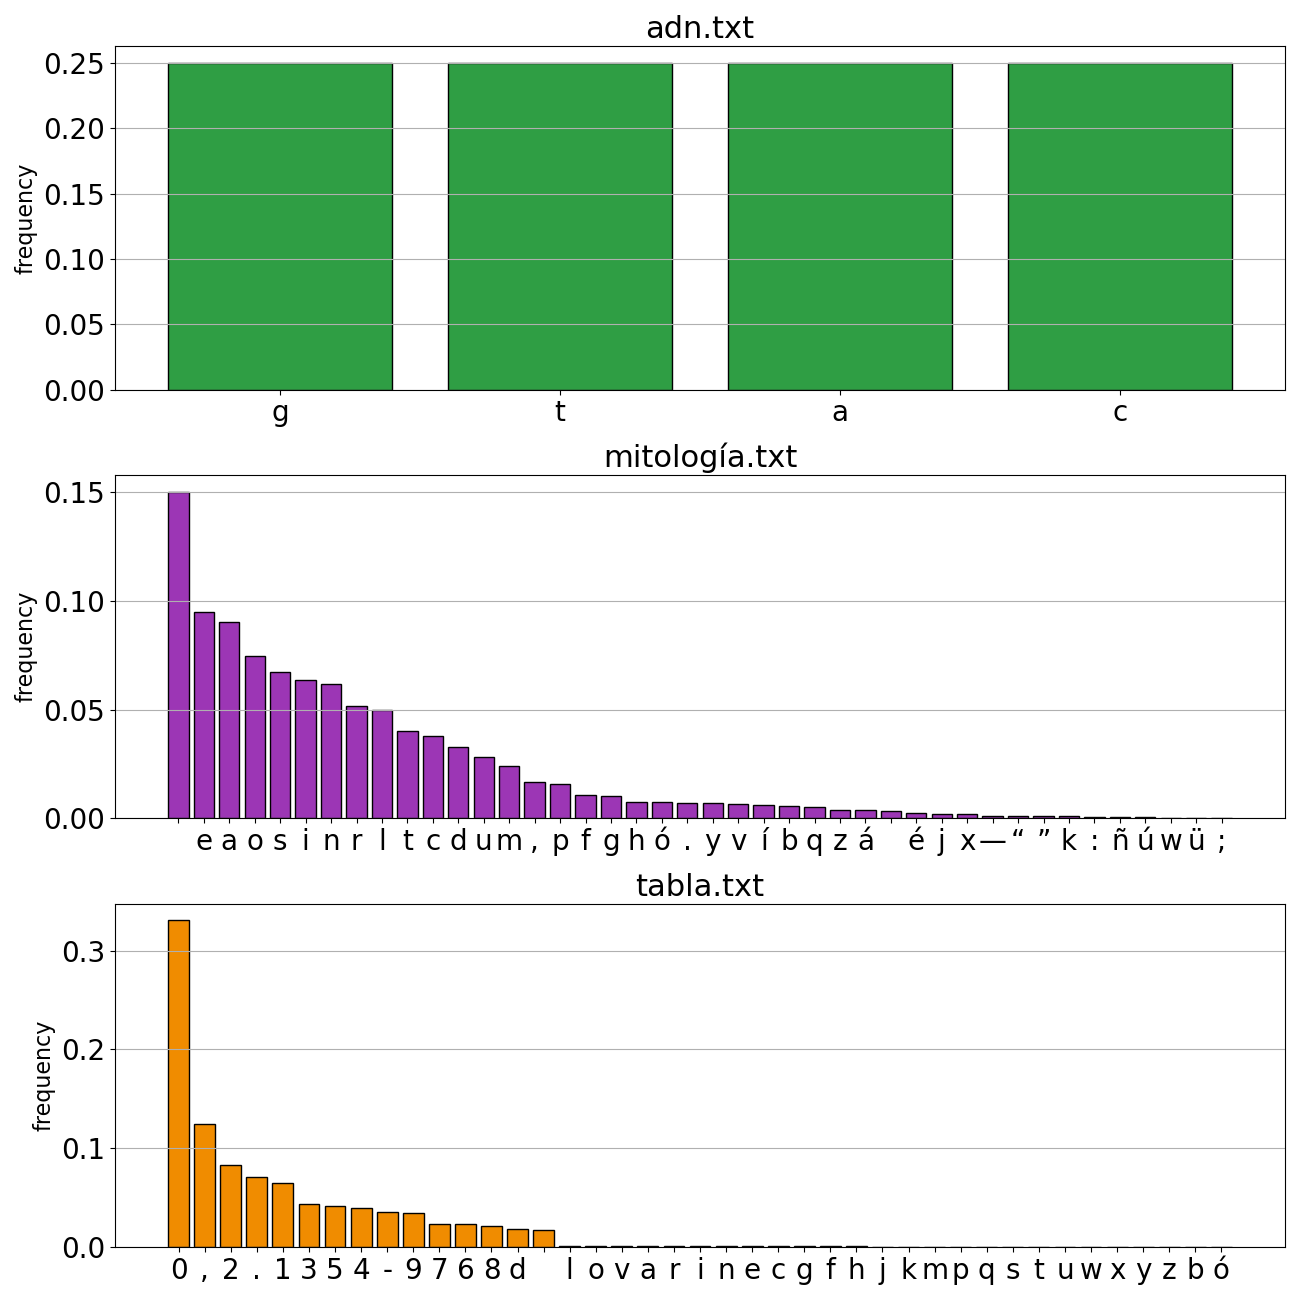
\includegraphics[width=0.41\textwidth]{figures/character_pmf.png}
    \caption{Masa de probabilidad de los caracteres para cada uno de los textos de ejemplos}
    \label{fig:character_pmf}
\end{figure}



Por otro lado, el archivo mitologia.txt muestra una distribucion de frecuencias muchos mas variadas. Notamos como unas pocas letras concentran una gran cantidad de las apariciones. Esto podria
deberse a la estructura del lenguaje español. Asimismo, vemos como el caracter mas usado es el ``\_'' (espacio) lo que concuerda con la regla gramatical de separar las palabras con este simbolo. {\color{red}(Capaz puede decir algo mas)}

Finalmente, en el ultimo archivo al ser una tabla de valores observamos como predominan los caracteres numericos y signos de puntuacion. A diferencia del caso anterior, esta distribucion no sigue parametros linguisticos sino de 
organizacion tipica de informacion numerica. 

En conjunto, estas diferencias exhiben como las distribuciones de frecuencia estan fuertemente determinados por la naturaleza de la informacion

Los tres textos presentan comportamientos muy distintos, lo que permite observar como la estructura estadistica mencionada anteriormente
influye directamente en su compresibilidad

El archivo adn.txt representa el extremo mas simple. Su distribucion uniforme produce una entropia baja de 1.99 bit/simbolo (1 normalizada) y una longitud promedio
de Huffman igual a la minima posible (2 bits/simbolo). Ante la inexistencia de diferencias en las probabilidades, el codigo no puede optimizarse, por lo que resulta en una reduccion de memoria nula.
Este es el peor caso posible donde la codificacion de Huffman no ofrece ninguna ventaja.

Por otra parte, la distribucion variada de mitologia.txt tipica del lenguaje natural genera una entropia intermedia 4.26 bits/simbolo (0.79 normalizada), y permite al algoritmo asignar codigos mas cortos a los simbolos frecuentes. Gracias a esto,
se obtiene una longitud promedio de 4.27 bits/simbolo y una reduccion de memoria de al 28.31\%. En este caso se puede apreciar claramente como la redundancia del lenguaje natural puede aprobecharse
para comprimir informacion de manera eficiente.

Por su parte, tabla.txt es aquel en el que se logra una mayor compresibilidad siendo de 41.30\%. Esto debido a que su frecuencia esta dominada por unos pocos caracteres numericos y signos de puntuacion. Esta fuerte concentracion reduce la entropia
a solo 3.46 bits/simbolo (0.64 normalizada) y permitiendo obtener la mayor eficiencia de codificacion.

\end{multicols}

%%%%%%%%%%%%%%%%%%%%%%%%%%%%%%%%%%%%%% Conclusión %%%%%%%%%%%%%%%%%%%%%%%%%%%%%%%%%%%%%%

\section{Conclusión}

    \begin{multicols}{2}

    \end{multicols}

\end{document}